\section{Implementation}

In this section, we will take a closer look at how the implementation works (Fig.~\ref{implementation}). Starting from the Client and following to the Providers, we show how we add the components in each application, what extra code we use to enable different authentication and authorization schemes.


\subsection{The Client}

The client is a Django application with a custom user model. Django comes with a user authentication system. It handles user accounts, groups, and permissions, using cookie-based user sessions. For authenticating, Django searches for the given user's credentials in its backends, and if the user exists, Django authenticates and redirects the user to the proper URL. We implement 2 custom backends for the Client application, one for searching users in the OAuth Provider (Fig.~\ref{oauth-backend}) and one for OIDC Provider (Fig.~\ref{oidc-backend}).

We installed the Python \textbf{django-social-auth}~\cite{djangosocial} module, which is a package for authenticating against third-party applications, like GitHub, Google, Facebook, and other websites. It also contains the base class for the OAuth authentication backend, called BaseOAuth2. In our custom OAuth backend, we override some of the BaseOAuth2 components, so the backend knows where to search for the Authorization Server, where to get the token, and other details.

For the OIDC custom backend, all we need to do is to overwrite the OpenIdConnectAuth class, defined by django-social-auth, provide the name of our backend and the URL of the Authorization Server. The Client is ready to redirect the Resource User to the Providers and initiate the OAuth/OIDC process.


\begin{figure}[htb]
	\centering
	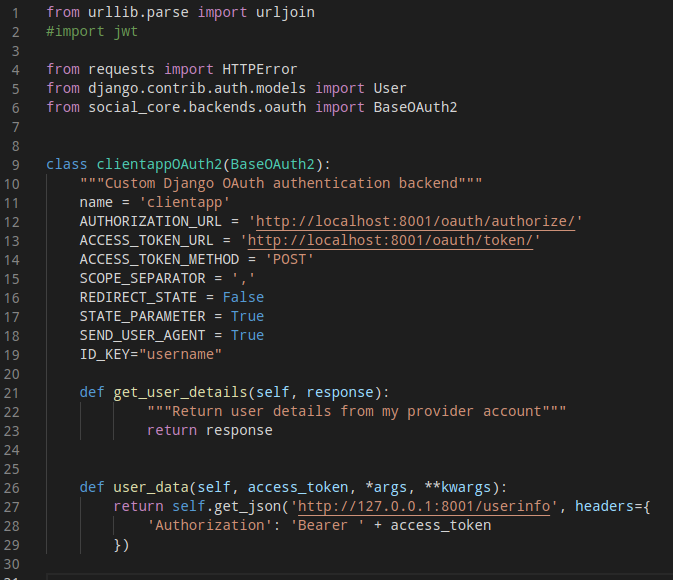
\includegraphics[scale=0.6]{figures/clientapp.png}
	\caption{OAuth custom backend}\label{oauth-backend}
\end{figure}


\begin{figure}[htb]
	\centering
	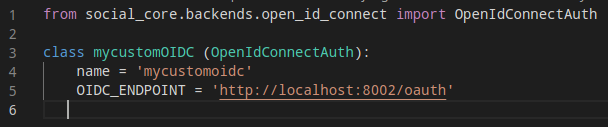
\includegraphics[scale=0.6]{figures/customOIDC.png}
	\caption{OIDC custom backend}\label{oidc-backend}
\end{figure}


\subsection{The Providers}

As mentioned, we used the Django-OAuth-Toolkit for the implementation of the Providers. To enable the Django-OAuth-Toolkit we need to add \verb|"oauth2_provider"| in installed apps and add the middleware \verb|"oauth2_provider.middleware.OAuth2TokenMiddleware"| in settings.py. The next step is to add the toolkit's backend for OAuth requests by adding:\linebreak
\verb|"oauth2_provider.backends.OAuth2Backend"| in authentication backends, and specifying the scopes as:\\
\verb|'SCOPES': {'read': 'Read scope', 'write': 'Write scope'}|.
In urls.py we add an extra URL: \verb|path('userinfo', user_info_secret)|, which is the endpoint in order for the custom backends to know where to search for the user's information after authenticating. We also provide the OAuth Toolkit's endpoints by adding \verb|url(r"^oauth/", include| \verb|('oauth2_provider.urls', namespace='oauth2_provider'))|.


For the OIDC Provider implementation, we need to do two more steps. Add the specific scope of \textbf{openid} in \verb|'SCOPES'|, and create a \verb|CustomOAuth2Validator| method, which is used for mapping the user's info from the OIDC Provider to the Client.



Finally, we have to register the Client in both of the Providers and set the correct Client\_id and Client\_secret in Client's settings.py. For the OIDC implementation, we need to provide an algorithm, which is used for signing the JWT that the Provider sends back to the Client, for which we used the RS256 algorithm. After the registration process, Providers are ready to give Access Tokens to the Client.

In the OIDC implementation, we also add the LDAP authentication scheme, by setting:

\begin{itemize}

	\item \verb|AUTH_LDAP_SERVER_URL|: Points to the LDAP server.

	\item \verb|AUTH_LDAP_BIND_DN|: Username.

	\item \verb|AUTH_LDAP_BIND_PASSWORD|: Password.

	\item \verb|AUTH_LDAP_USER_DN_TEMPLATE|: How to find the user.

	\item \verb|AUTH_LDAP_USER_ATTR_MAP|: What attributes we want to populate the Django user who is going to be created.

\end{itemize}

The whole implementation is shown in Fig.~\ref{implementation}. The Resource Owner wants to use the Client which is a Django application with two custom backends and can authenticate the user via the OAuth or OIDC implementation of the Provider. The OAuth and OIDC Providers are Django apps and use the Django-oauth-toolkit.


\begin{figure}[htb]
	\centering
	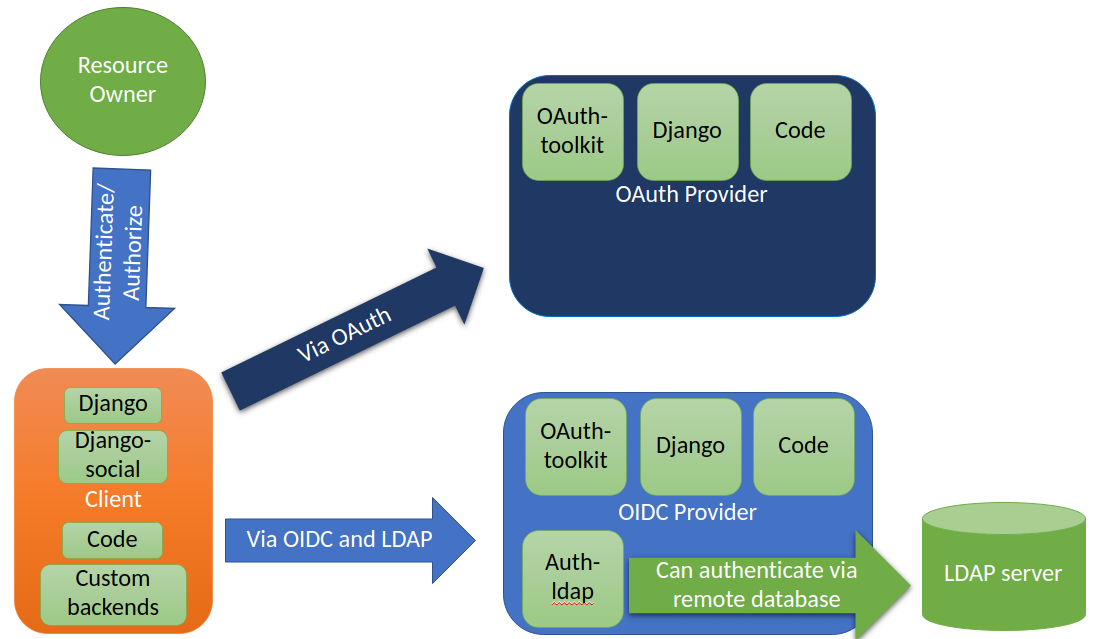
\includegraphics[scale=0.4]{figures/implementation.png}
	\caption{Implementation}\label{implementation}
\end{figure}

